%%=====================================================================================
%%
%%       Filename:  data-structs-and-algs.tex
%%
%%    Description:  Formal notes of DS and A
%%
%%        Version:  1.0
%%        Created:  02/10/19
%%       Revision:  none
%%
%%         Author:  Josh Felmeden (), nk18044@bristol.ac.uk
%%   Organization:  
%%      Copyright:  Copyright (c) 2019, Josh Felmeden
%%
%%          Notes:  
%%
%%=====================================================================================

% Preamble {{{
\documentclass[11pt,a4paper,titlepage,dvipsnames,cmyk]{scrartcl}
\usepackage[english]{babel}
\typearea{12}
% }}}

% Set indentation and line skip for paragraph {{{
\setlength{\parindent}{0em}
\setlength{\parskip}{1em}
\usepackage[margin=2cm]{geometry}
\addtolength{\textheight}{-1in}
\setlength{\headsep}{.5in}
% }}}

\usepackage{hhline} 
\usepackage{mathtools} 
\usepackage[T1]{fontenc}

% Headers setup {{{
\usepackage{fancyhdr}
\pagestyle{fancy}
\lhead{Data Structures and Algorithms: The formal notes}
\rhead{Josh Felmeden}
\usepackage{hyperref} 
% }}}

% Listings {{{
\usepackage[]{listings,xcolor} 
\lstset
{
    breaklines=true,
    tabsize=3,
    showstringspaces=false
}

\definecolor{lstgrey}{rgb}{0.05,0.05,0.05}
\usepackage{listings}
\makeatletter
\lstset{language=[Visual]Basic,
    backgroundcolor=\color{lstgrey},
    frame=single,
    xleftmargin=0.7cm,
    frame=tlbr, framesep=0.2cm, framerule=0pt,
    basicstyle=\lst@ifdisplaystyle\color{white}\footnotesize\ttfamily\else\color{black}\footnotesize\ttfamily\fi,
    captionpos=b,
    tabsize=2,
    keywordstyle=\color{Magenta}\bfseries,
    identifierstyle=\color{Cyan},
    stringstyle=\color{Yellow},
    commentstyle=\color{Gray}\itshape
}
\makeatother
\renewcommand{\familydefault}{\sfdefault}
% }}}


% Other packages {{{
\usepackage{amssymb}
\usepackage{graphicx}
\graphicspath{ {./pics/} }
\usepackage{needspace}
\usepackage{tcolorbox}
\usepackage{soul}
\usepackage{babel,dejavu,helvet} 
\usepackage{amsmath} 
\usepackage{booktabs} 
\usepackage{tcolorbox} 
\usepackage[symbol]{footmisc} 
\renewcommand{\thefootnote}{\fnsymbol{footnote}}
\renewcommand{\familydefault}{\sfdefault}
% }}}

% Title {{{
\title{Data Structures and Algorithms: The formal notes}
\author{Josh Felmeden}
% }}}

\begin{document}

\maketitle
\tableofcontents

\newpage
\section{Greedy algorithms}%
\label{sec:Greedy algorithms}
\subsection{Interval scheduling}%
\label{sub:interval-scheduling}
Let's suppose that you're running a satellite imaging service. Taking a
satellite picture of an area isn't instant and can take some time. It can
also only be done on the day where the satellite's orbit is lined up
correctly. Say you want to request some images to be taken from said
satellite, each of which can only be taken at certain times and you can
only take one picture at a time. How do we satisfy as many requests as
possible?

The requested satellite times that we have to deal with are: 12:00-12:30,
12:05-12:20, 12:15-12:55, 12:20-12:25, 12:38-12:50, and 12:45-13:00.

If we visualise this in a graph, we get: 


\begin{center}
    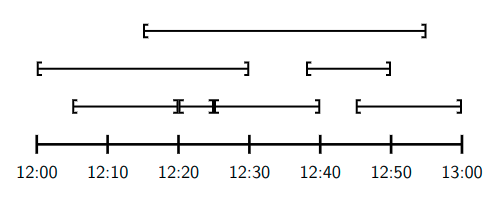
\includegraphics[scale=.5]{graph-satellite.png}
\end{center}

If we take a greedy algorithm approach to assigning these slots, we could
do something like assign the slot that finishes earliest, and then repeat
doing this until we have reached the end. For example, the slot that
finishes fastest is 12:05-12:20, so we assign this. This now removes the
ability for both 12:10-12:30 and 12:15-12:55 to be assigned, so we remove
these. This continues until we end up with something looking like this:


\begin{center}
    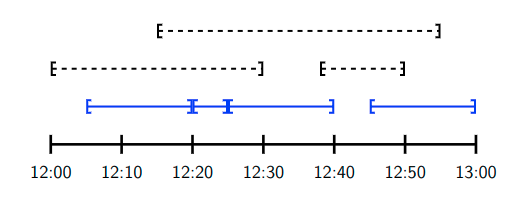
\includegraphics[scale=.5]{graph-assigned}
\end{center}

This means that we satisfy four requests (which is actually the maximum
possible, so well done us).

We can formalise this by saying that a \textbf{request} is a pair of
integers $(s,f)$ with $0 \le s \le f$.

\newpage
The algorithm that we're left with is this:
\begin{lstlisting}
public sub greedySchedule
    sort R
    for each i in {1 ... n} do
        if s_i >= lastf then
            A.append(s_i, f_i)
            lastf = f_i
        end if
    next
end sub
\end{lstlisting}

Now, we need to prove that the output is actually a \textbf{compatible
subset} of R. This is sort of intuitive because the set we added doesn't
break compatibility, since $s \ge$ \lstinline|lastf| and \lstinline|lastf|
is the latest finish time that's already in $A$.

We can formalise this with a loop invariant. At the start of the $i$th
iteration, we see that
\begin{itemize}
    \item $A$ contains a compatible subset $\{(S_1,F_1), \dots,
        (S_t,F_t)\}$ of R.
    \item \lstinline|lastf| = $\max(\{0\} \cup \{F_j : j \le t\})$ 
\end{itemize}

The base case ($i=0$) is immediate because $A = []$. The induction step is
that $A$ was compatible at the start of the iteration, and therefore if we
append a pair $s_i,f_i$ to $A$ then $s \ge $ \lstinline|lastf| $\ge F_j$
for all $f \le t$. This means that $(s_i,f_i)$ is compatible with $A$.


\begin{tcolorbox} [space to upper,
        collower=white,
        title={Greedy algorithm definition},
        nobeforeafter,
        halign lower=flush right, ]
Greedy algorithms are actually an informal term and people have different
definitions. The definition that we're going to use is:
\begin{itemize}
    \item They start with a sub-optimal solution.
    \item They look over all the possible improvements and pick the one
        that looks the best at the time.
    \item They never backtrack in `quality'.
\end{itemize}
\end{tcolorbox}

Greedy algorithms might fail; it's not enough to just do the obvious thing
at each stage. While the algorithms might fail initially, we can use the
knowledge that we gained from the results of the algorithm to design a
more correct one.

\section{Graphs}%
\label{sec:Graphs}

\begin{tcolorbox} [space to upper,
        collower=white,
        title={Graph definition},
        nobeforeafter,
        halign lower=flush right, ]
        A \textbf{graph} is a pair $G = (V,E)$ where $V=V(G)$ is a set of
        \textbf{vertices} $E = E(G)$ is a set of \textbf{edges} contained
        in $\{\{u,v\} : u,v \in V, u \not = \}$
\end{tcolorbox}

\begin{tcolorbox} [space to upper,
        collower=white,
        title={Walk definition},
        nobeforeafter,
        halign lower=flush right, ]
        A \textbf{walk} in a graph $G = (V, E)$ is a sequence of vertices
        such that $\{v_i, v_{i+1} \in E for all i\le k-1$

        We say that the walk is from $v_0$ to $v_k$ and call $k$ the
        length of the walk.
\end{tcolorbox}


\subsection{Euler walks}%
\label{sub:Euler walks}
An \textbf{Euler walk} is one that contains every edge in $G$
exactly once.

Two graphs might be \textbf{equal}. This is the case when two graphs $G_1
= (V_1, E_1)$ and $G_2 = (V_2, E_2)$ are equal and written $G_1 = G_2$ if
$V_1 = V_2$ and $E_1 = E_2$. This does present some issues, however,
because sometimes graphs look like they should be equal, when they're not
because the edges are labelled differently.

This is where \textbf{isomorphism} comes in. $G_1$ and $G_2$ are
\textbf{isomorphic} if there's a bijection $f: V_1 \rightarrow V_2$ such
that $\{f(u),f(v) \} \in E_2$ if and only if $\{u,v\} \in E_1$.

Intuitively, this means that $G_1 \xrightarrow{\sim} G_2$ if they are the
same graph but the vertices are relabelled.

In a graph $G = (V,E)$, the \textbf{neighbourhood} of a vertex $v$ is the
set of vertices joined to $v$ by an edge. Formally, 
$N_G(v) = \{w \in V : \{v,w\} \in E$. Also, for all sets of vertices
$X \subseteq V = \cup_{v\in X} N_G(v)$

The \textbf{degree} of a vertex $v$ is the \textbf{number} of vertices
joined to $v$. Formally: $d_G(v) = |N_G(v)|$

\textbf{Theorem}: If $G$ has an Euler walk, then either:
\begin{itemize}
    \item Every vertex of $G$ has even degree or
    \item All but two vertices $v_0$ and $v_k$ have even degree, and any
        Euler walk must have $v_0$ and $v_k$ as endpoints.
\end{itemize}

Does every single graph that satisfies both of these conditions have an
Euler walk? No, because the graphs need to be \textbf{connected}.

Within a graph, we also have subgraphs and induced subgraphs. A
\textbf{subgraph} $H = (V_H, E_H)$ of $G$ is a graph with $V_H \subseteq$
and $E_H \subseteq E$. $H$ is an \textbf{induced subgraph} if $V_H
\subseteq V$ and $E_H = \{ e \in E : e \subseteq V_H\}$.

For all vertex sets $X \subseteq V$, the graph is \textbf{induced} by $X$
is:

\begin{center}
    \begin{align*}
        G[X] = (X, \{e \in E: e \subseteq X \})
    \end{align*}
\end{center}

A \textbf{component} $H$ of $G$ is the maximal connected induced subgraph
of $G$, so $H = G[V_H]$ is connected, but $G[V_H \cup \{v\}]$ is
disconnected for all $v \in V \backslash V_H$.




\end{document}
